\clearpage{\pagestyle{empty}\cleardoublepage}
\chapter{Linea di produzione di Verdicchio: tensioattivi per lo spiazzamento dell'acqua in condotta}\thispagestyle{empty} 
\chaptermark{Applicazione schiumogeno in condotta}
Il giorno venerdì 12 giugno 2015 è stato effettuato il test di campo del foamer Chimec  Phoenix 6163 presso il campo SNM. Dopo l''esperienza tra il 23 e il 27 febbraio 2015 presso il pozzo CZT-2d, obiettivo primario del test è stato quello di spiazzare l'acqua dalla linea San Marco (lunghezza 13,6 km, diametro 4"), così da diminuire le cadute di pressione e favorire la produzione dei pozzi a monte.
I risultati ottenuti sono stati:
\begin{itemize}
	\item acqua spiazzata: 12,74 m\ap{3}
	\item tempo impiegato: 2h10m
	\item pressione minima: 5,5 bar
\end{itemize}
I tempi di spiazzamento, estremamente brevi, sono collegati al comportamento del foamer. Grazie alla conformazione della mandata e  alla miscela con acqua, il tensioattivo ha agito come un "pig" chimico, capace di spiazzare l'acqua dalla condotta con conseguente guadagno in termine di tempo e praticità.

\section{Polo produttivo di San Giorgio Mare}
La centrale di San Giorgio Mare (centrale SGM), collocata nel Comune di Fermo in Località Marina Palmense (FM), è destinata all'attività di produzione, compressione e trattamento di gas naturale ed è stata sviluppata a cavallo tra il 1970 e il 1972. L'impianto rientra nella Business Unit Asset Idrocarburi della Edison S.p.A. ed è gestito dal Distretto Operativo di Sambuceto (CH) che cura inoltre la Direzione di tutte le attività del Sistema di Gestione Integrato dell'Ambiente e della Sicurezza. Il polo produttivo di San Giorgio Mare comprende:
\begin{itemize}
	\item pozzi relativi alle concessioni off-shore di Vongola Mare (VGM1), San Giorgio Mare (SGMC, SGM3, SGM6) e concessioni in-shore Verdicchio (VRD-1), San Marco (SNM1-2-3), Cozza Terra (CZT-2D), Cassiano1D, Castellaro 1;
	\item linee di collegamento tra pozzi e centrale SGM;
	\item centrale SGM;
	\item vasche e serbatori di raccolta acque e gasolina;
	\item punti di collegamento con le reti di distribuzione a carattere nazionale (Snam Rete Gas e SGI S.p.A.).
\end{itemize}
La centrale SGM riceve il gas proveniente dai pozzi e le piattaforme off-shore mediante una tubazione sottomarina (\textit{sealine}) da 8" di diametro o da 8 NPS (\textit{Nominal Pipe Size}, dimensione nominale della condotta), e 10 NPS dal campo SGM. Il gas proveniente dai campi on-shore arriva in centrale tramite condotta sotterrata da 6 NPS. Recentemente la centrale MAM è stata collegata alla rete on-shore dove, tramite una condotta da 4 NPS, convoglia il gas associato alla produzione  di olio di Sarago Mare (SGM).

\begin{landscape}
	\begin{figure}[htbp]
    	\centering
    	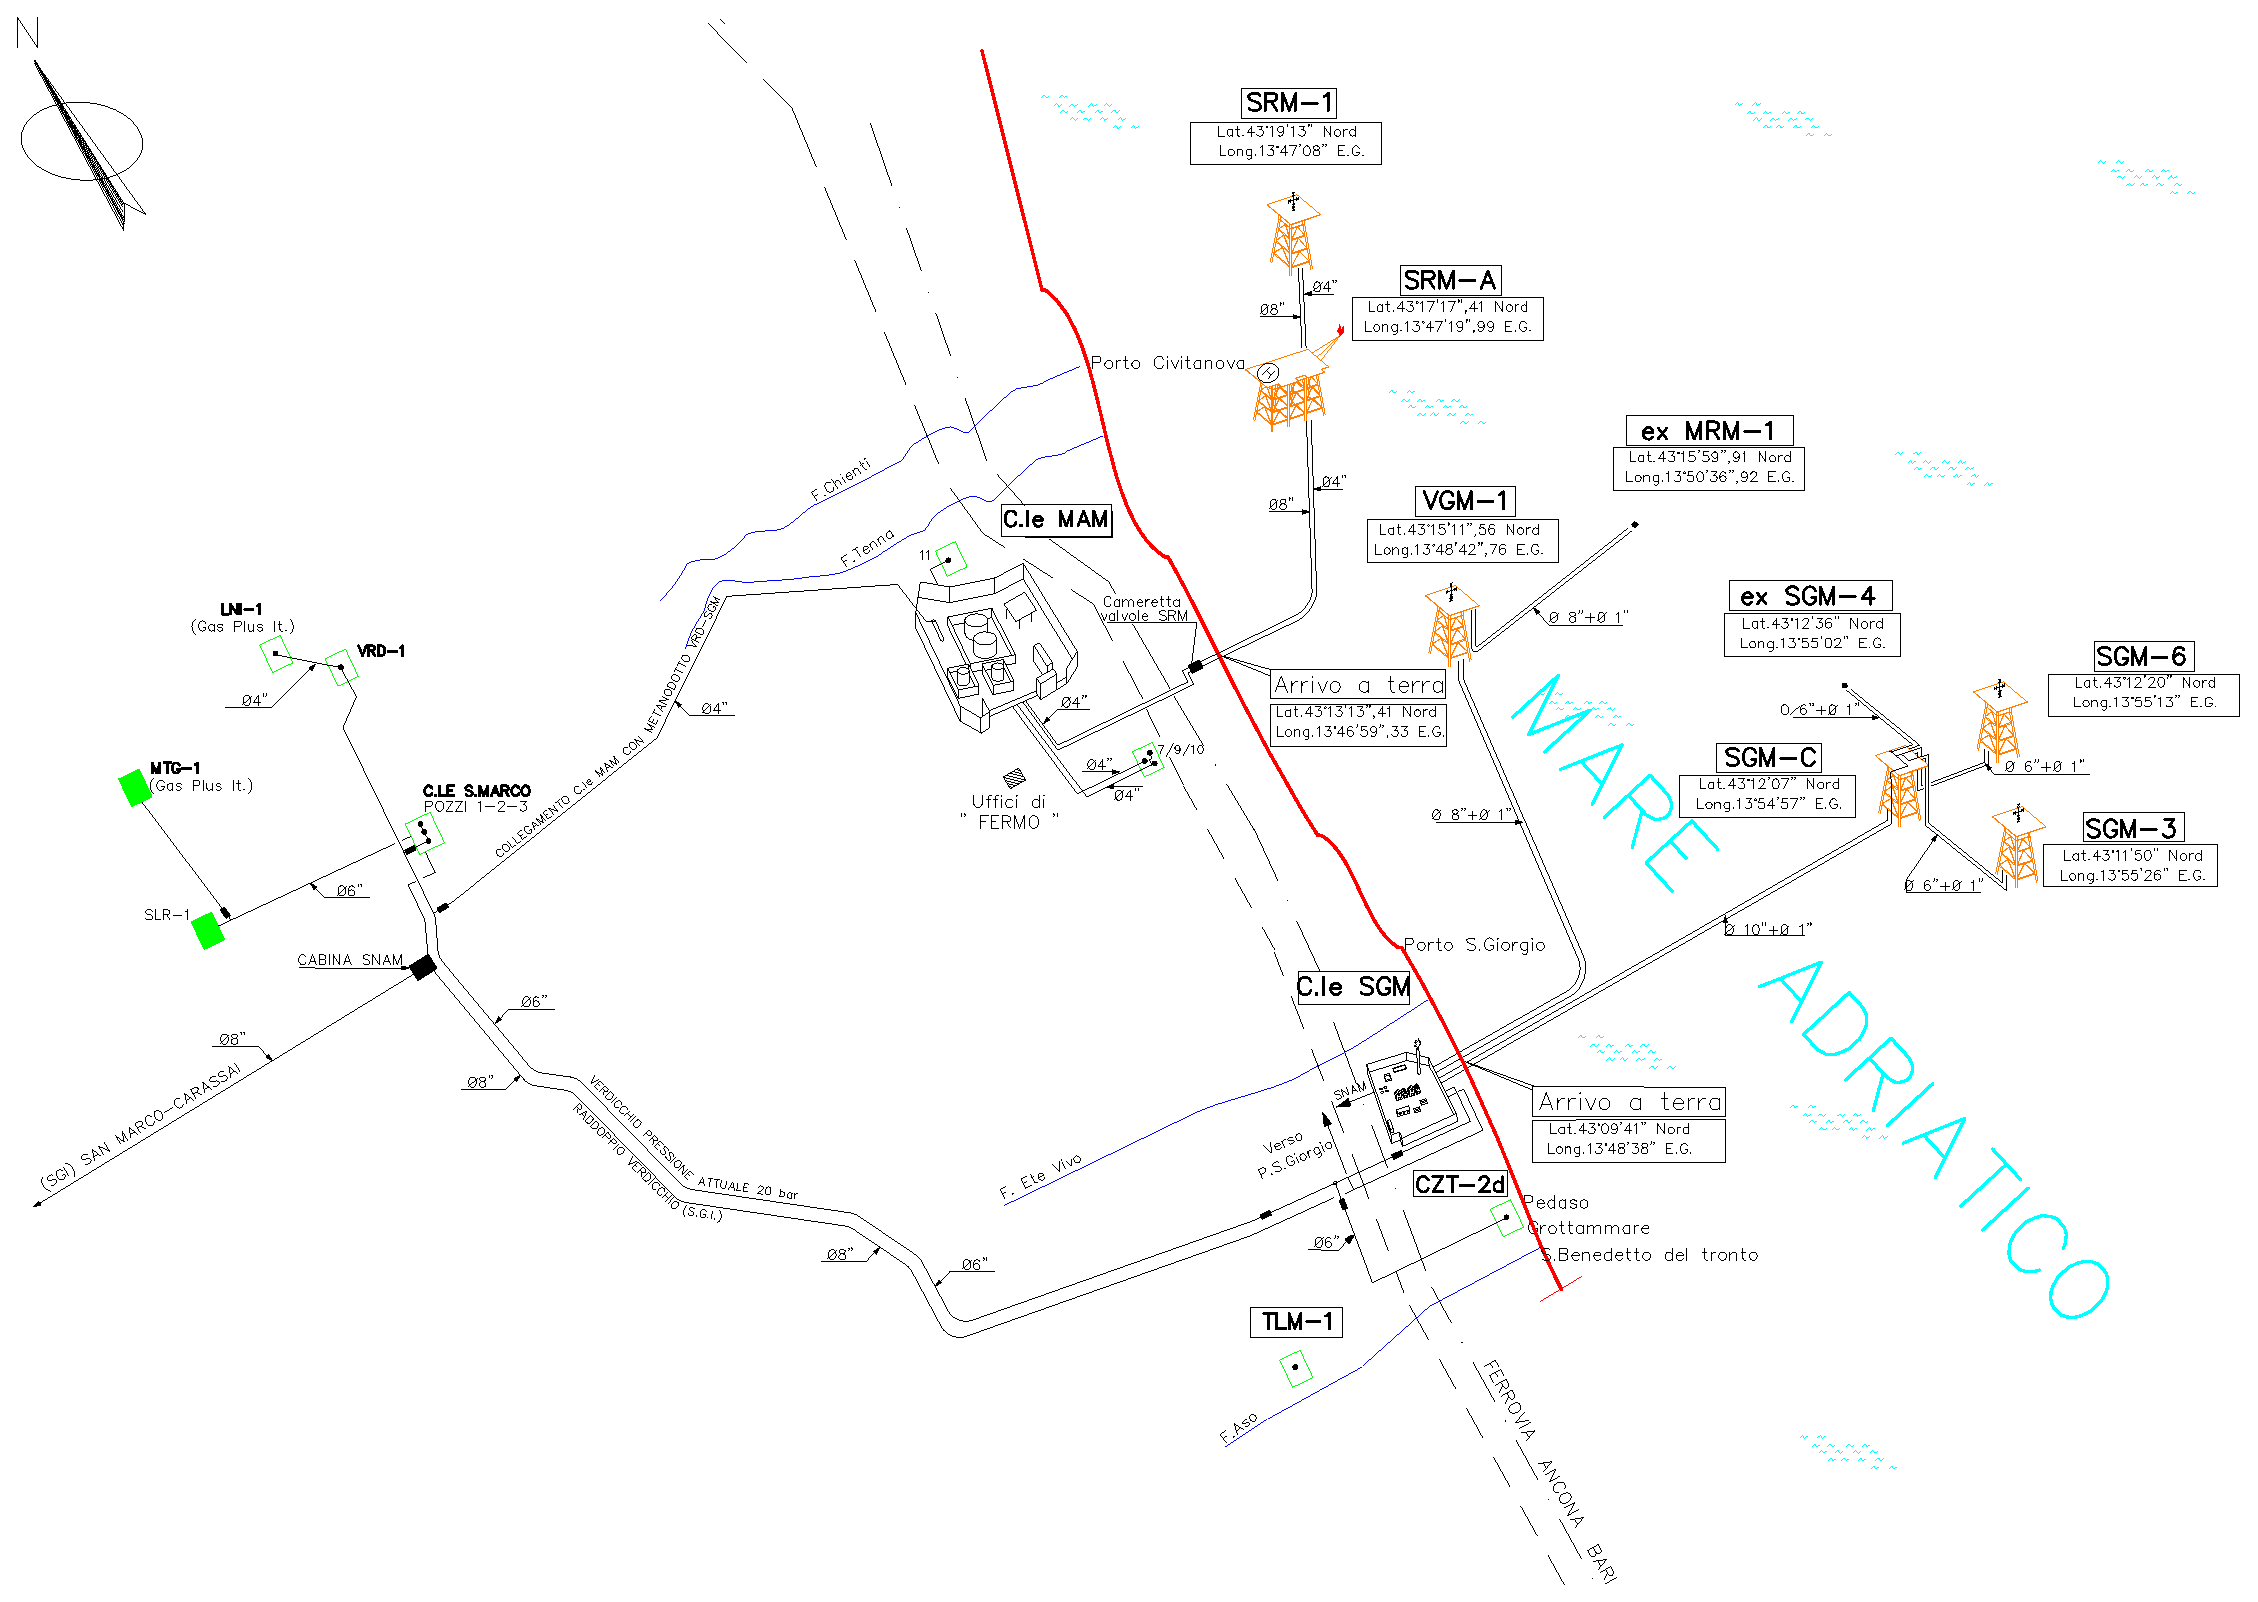
\includegraphics[width=\textwidth]{fig/test/asset.eps}
    	\caption{Planimetria delle installazioni on-shore e off-shore relative al polo produttivo di San Giorgio Mare.}
    	\label{fig:asset}
	\end{figure}
\end{landscape}

\subsection{Descrizione delle aree pozzo interessate}
\subsubsection{Verdicchio}
\subsubsection{San Marco}

\subsection{La centrale di San Giorgio Mare}
La centrale SGM si trova nel cuore del polo produttivo di San Giorgio Mare, nella Località Marina Palmense (FM), a circa 300 m di distanza dalla costa e 200 m dall'autostrada A14. L'area complessiva interessata è di circa 30.000 m\ap{2}, di cui 300 m\ap{2} dedicata agli uffici e alla sala controllo.
Le principali attività svolte dal polo produttivo di San Giorgio Mare sono:
\begin{itemize}
 	\item produzione di gas dal giacimento;
 	\item separazione dell'acqua e gasolina (principalmente dal pozzo SGM6) associate al gas naturale;
 	\item stoccaggio e spedizione dell'acqua di strato;
 	\item compressione del gas naturale;
 	\item disidratazione del gas naturale;
 	\item vendita del gas naturale, previa misura fiscale.
\end{itemize}

\subsubsection{Impianti di processo}
\paragraph{Separatori}
I separatori S-101, S-111, S-112 sono separatori orizzontali, S-101 e S-111 sono separatori bifase mentre S-112 è un separatore trifase, dedicato al gas a condensati proveniente dai campi off-shore di San Giorgio Mare. La geometria dei separatori è diversa e va da un volume minimo di S-101 pari 2.100 litri a un massimo di S-111 pari a 10.500 litri. L'acqua di strato viene  inviata tramite autobotti alla centrale MAM e pompata nei pozzi di reiniezione, come previsto da autorizzazione. La gasolina proveniente dal solo separatore S-112 è inviata all'impianto di trattamento dedicato.
La regolazione dei rispettivi livelli avviene tramite valvole di controllo livello (LCV, \textit{Level Control Valve}), mentre la pressione dei separatori è regolata tramite la valvola di controllo della pressione (PCV, \textit{Pressure Control Valve}).

\paragraph{Compressori}
L'impianto di compressione è cosituito da:
\begin{itemize}
	\item compressore (K-101 e K-202): motocompressori alternativi (monstadio a doppio effetto) della Nuovo Pignone. I cilindri sono lubrificati e il raffreddamento è ad acqua. Ogni compressore lavora con un rapporto di compressione di 1:3 e sono configurati in serie in modo tale da portare la pressione da 5-7 bar a 45-60 bar.
	\item motore compressore: motore Waukesha (General Electric) endodermico a ciclo Otto alimentato a gas, cilindrata totale da 115.400 cm\ap{3}. La potenza della macchina è di 1547 BHP (\textit{British Horse Power}, cavallo vapore britannico) a 1200 RPM (\textit{Revolutions Per Minute}, giri al minuto);
	\item aerorefrigerante (A-101 e A-201): impianto di raffreddamento ad aria della Nuovo Pignone che raffredda il gas una volta compresso. L'aerorefrigerante è costituito oltre che dalla sezione di refrigerazione del gas di processo anche da due sezioni per la refrigerazione delle acque ausiliarie.
\end {itemize}

\begin{figure}[htbp]
    \centering
    \subfloat[][Vista da Sud dell'impianto di compressione complessivo.]
    {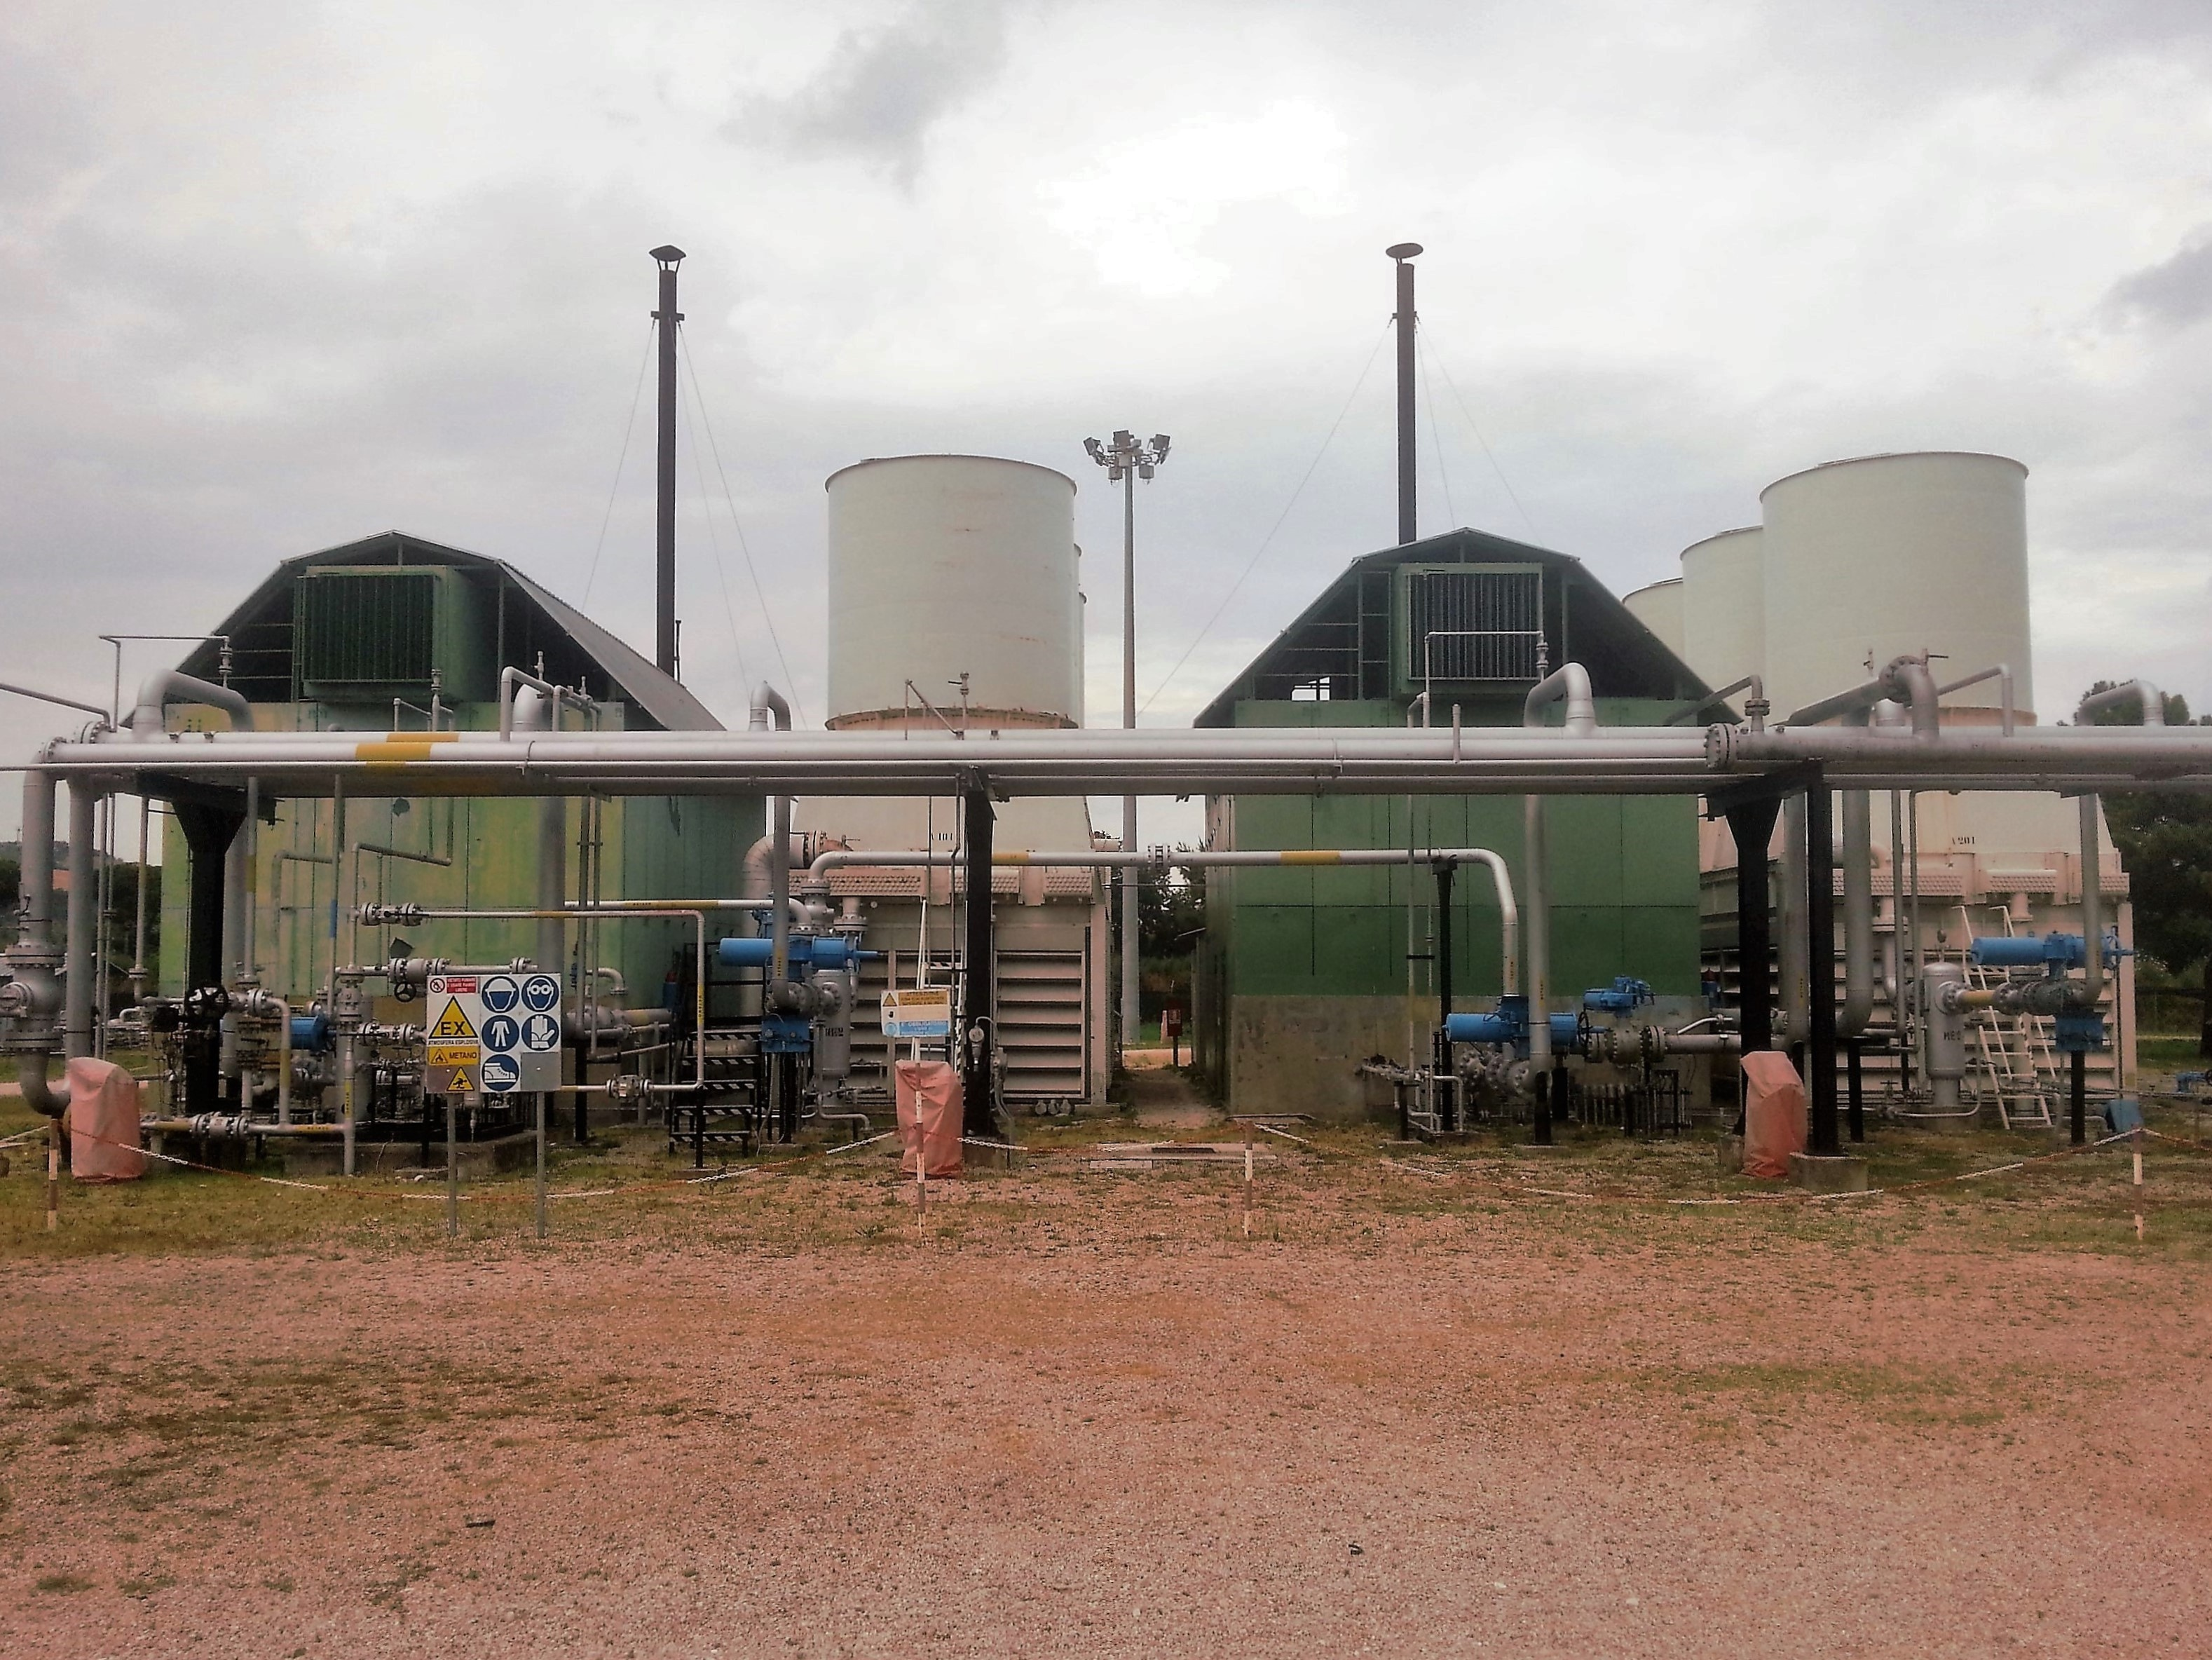
\includegraphics[width=\textwidth]{fig/test/centrale/compressori2.jpg} \label{fig:compressionegenerale}}\\
    \subfloat[][Impianto di raffreddamento ad aria A-201.]
    {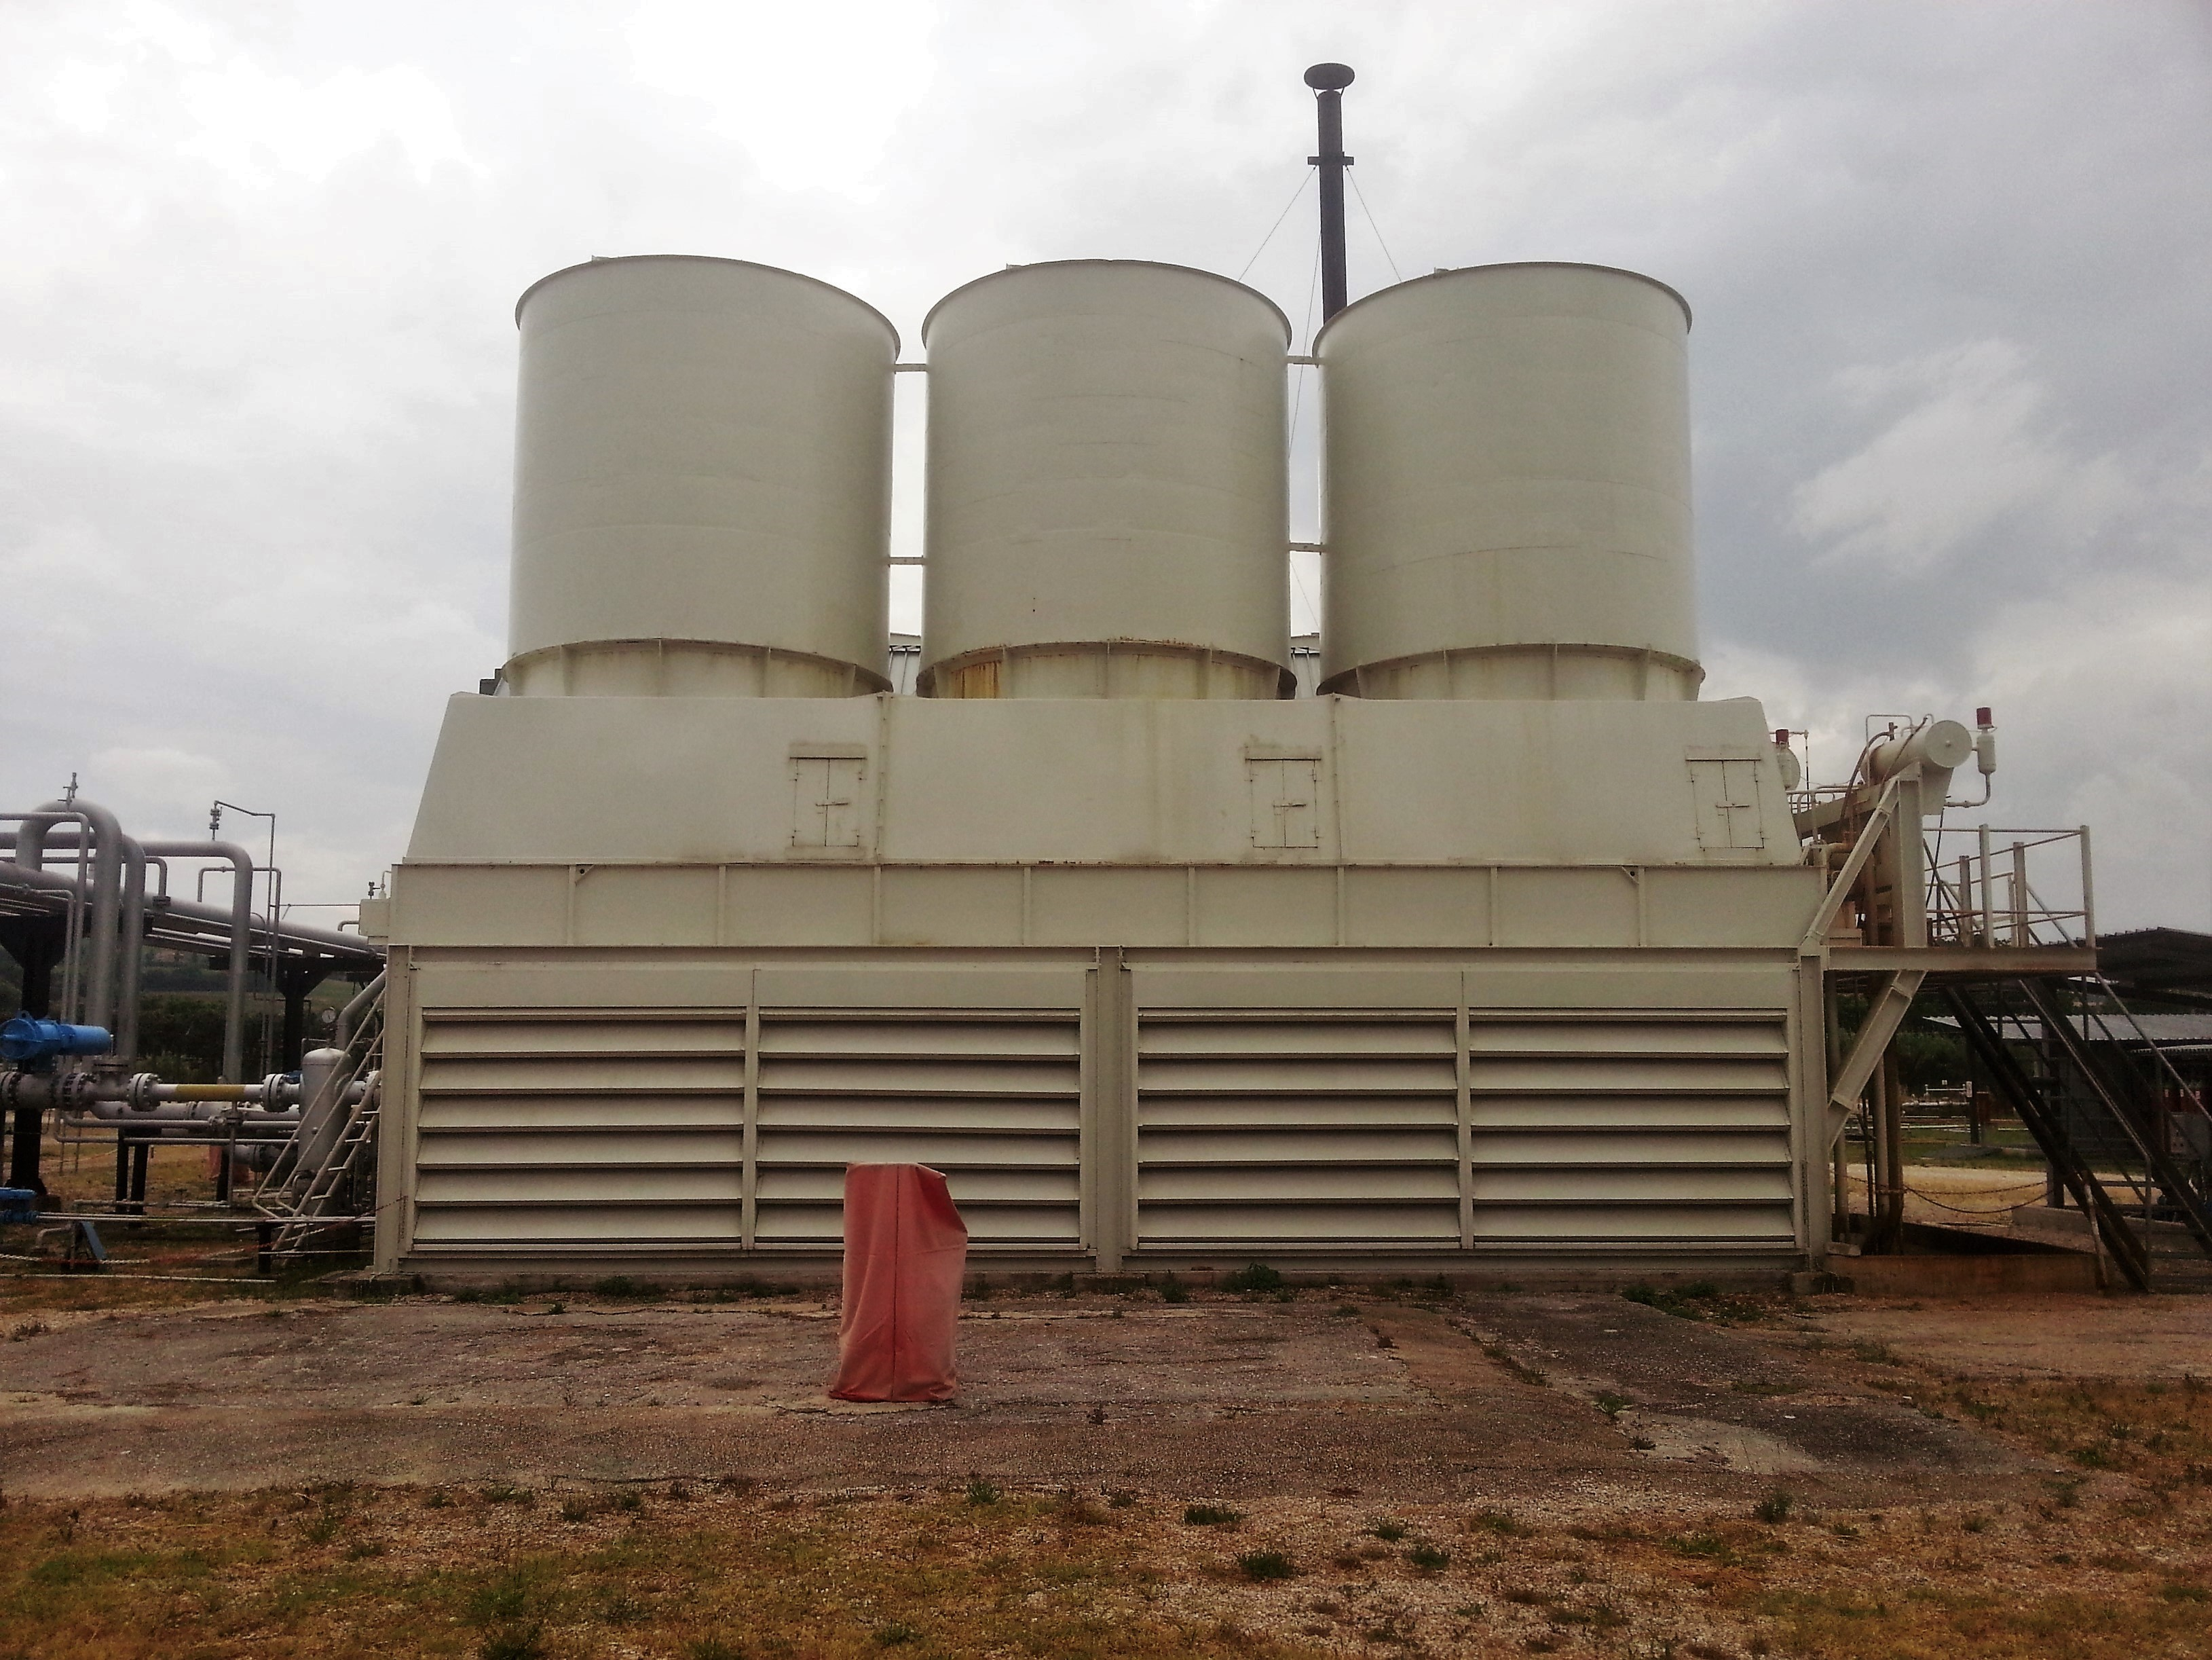
\includegraphics[width=.45\textwidth]{fig/test/centrale/compressori1.jpg} \label{fig:compressioneraffreddamento}} \qquad
    \subfloat[][Compressore K-201.]
    {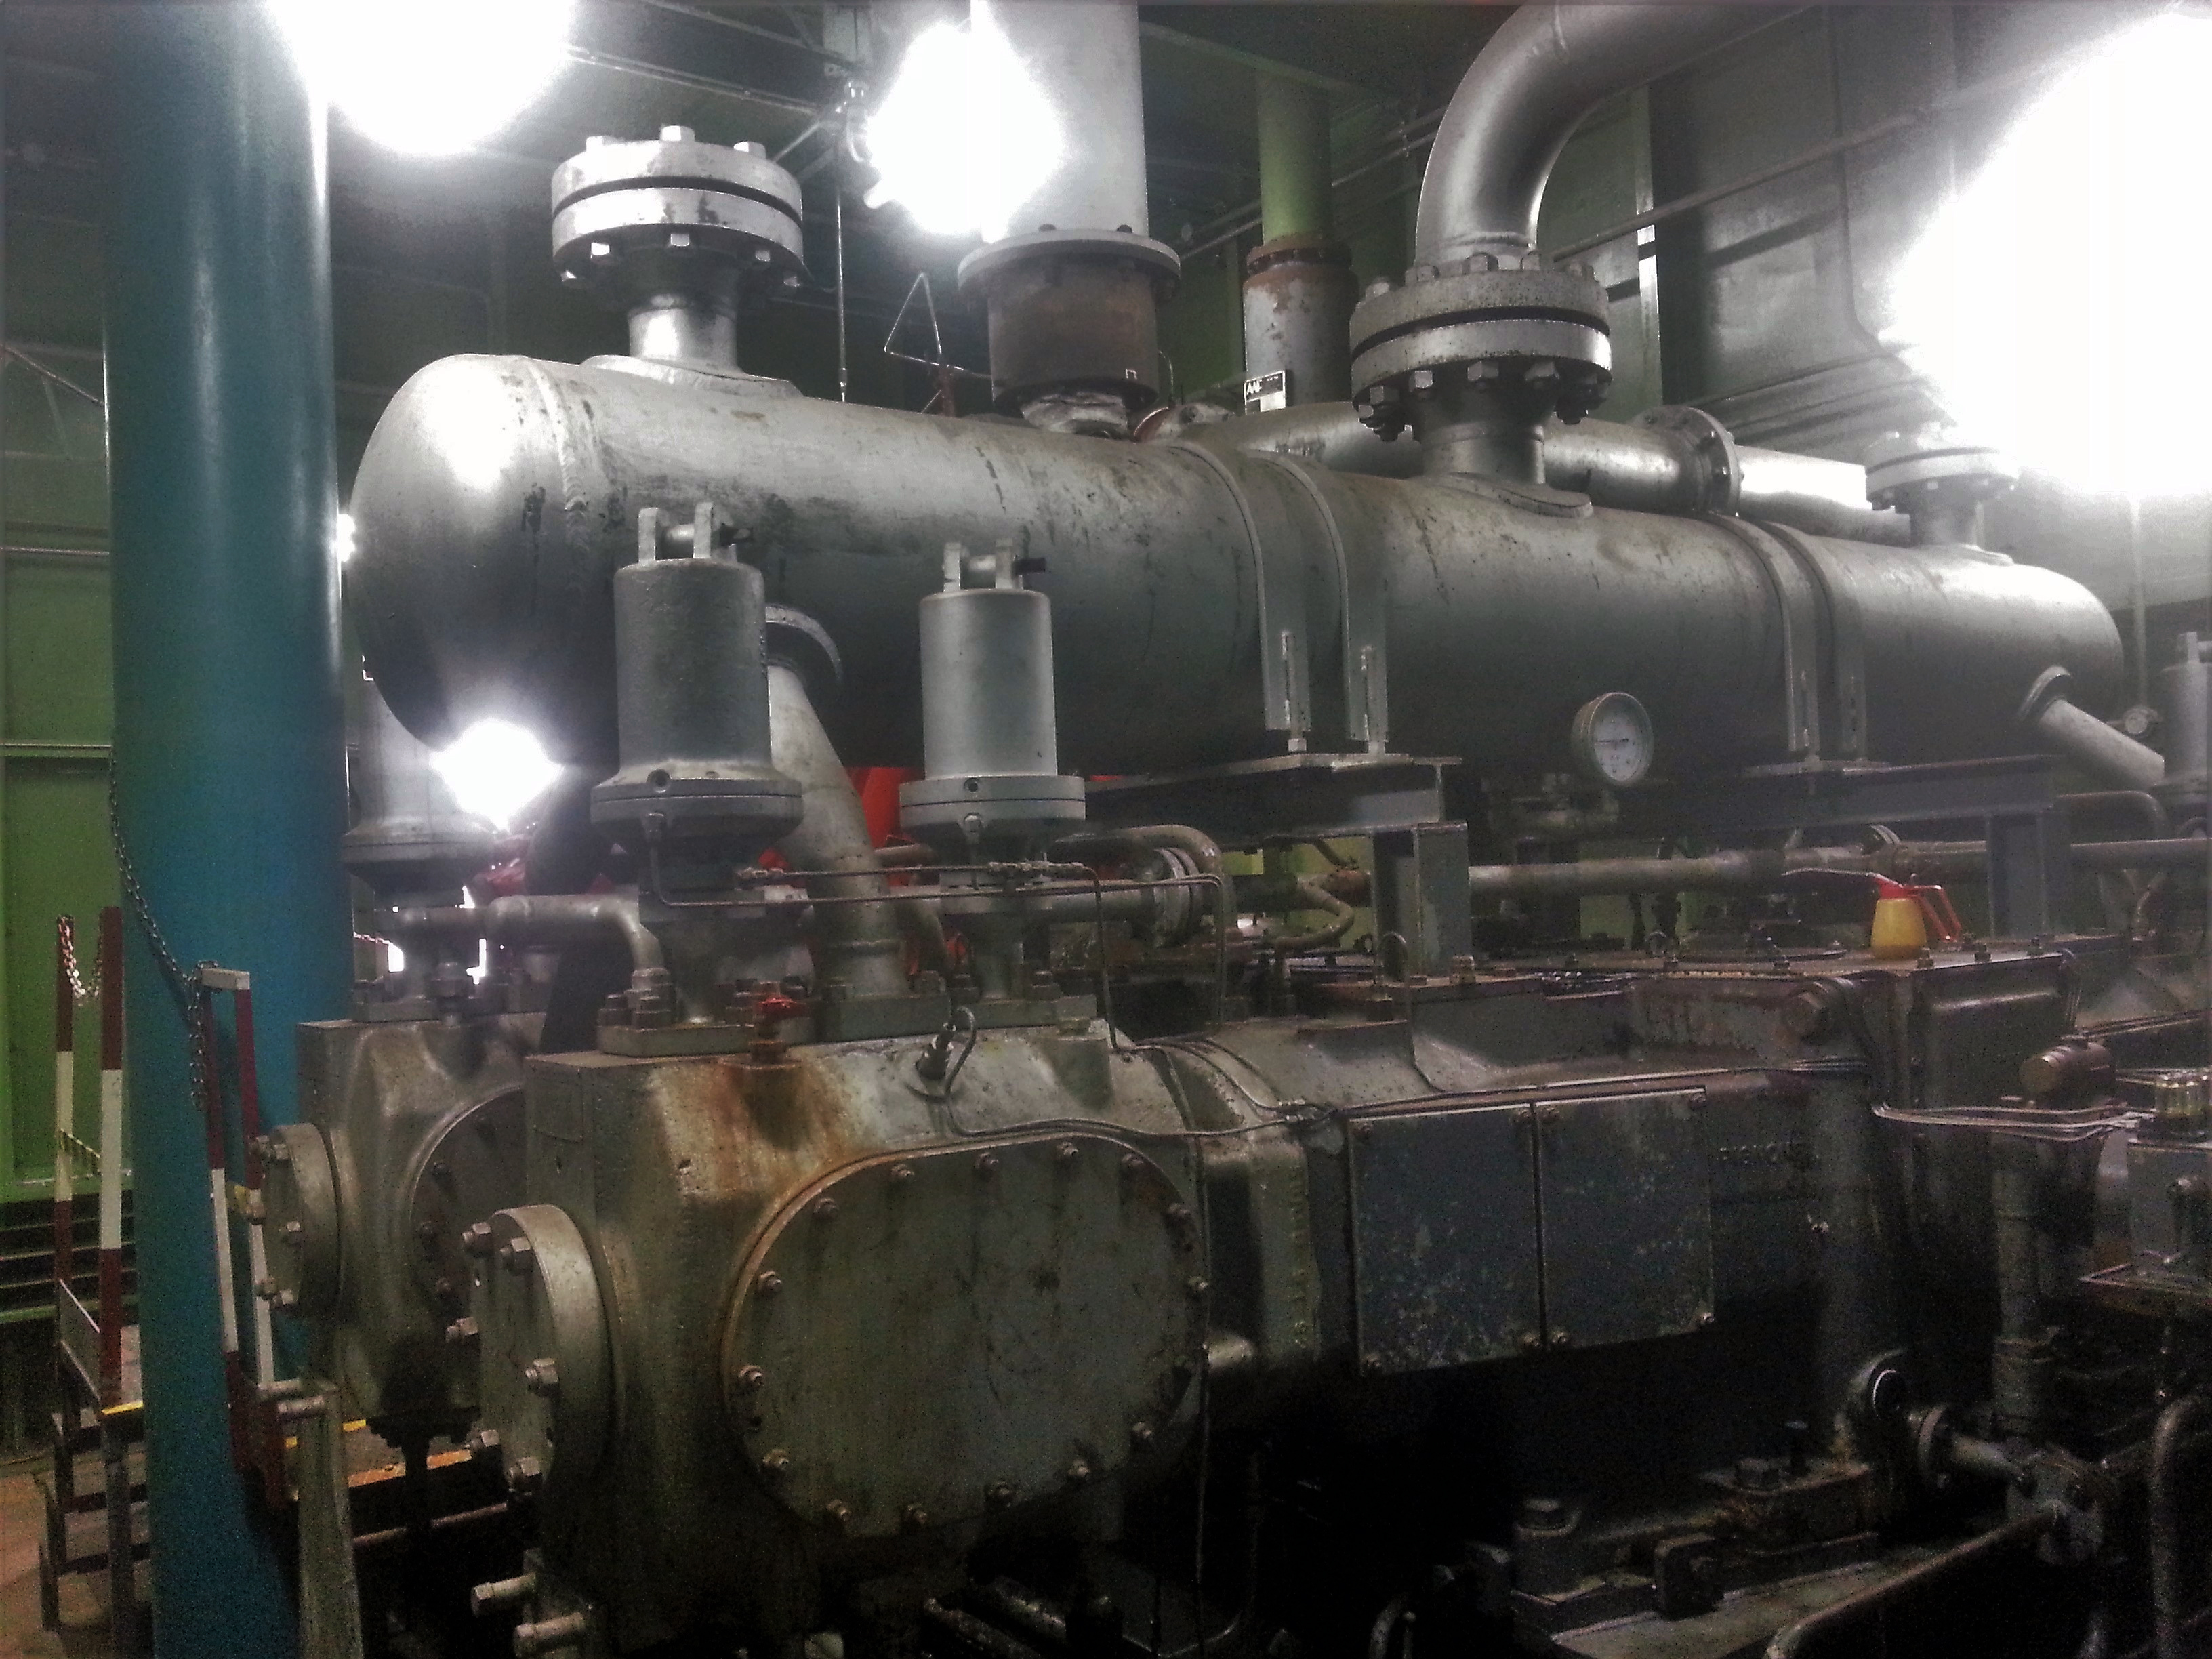
\includegraphics[width=.45\textwidth]{fig/test/centrale/compressori4.jpg} \label{fig:compressa}}   
\caption{Impianto di compressione del gas naturale, centrale SGM.}
\label{fig:centrale-compressione}
\end{figure}

\paragraph{Unità di condensazione a bassa temperatura}
La disidratazione e degasolinaggio avviene a opera di un unità di condensazione a bassa temperatura. L'impianto è del tutto equivalente a un LTS convenzionale, al quale però è aggiunto uno scambiatore gas-freon associato a unità frigorifera poiché le pressioni in ingresso in centrale non sono sufficienti a garantire una differenza di pressione sulla duse tale da raggiungere le temperature desiderate in camera di espansione. L'unità di condensazione è costituita da:
\begin{itemize}
	\item \textbf{scambiatore gas/gas}: costituito da due cilindri da 16" di diametro e 24 ft di lunghezza in seria, superficie di scambio totale di 162 m\ap{2}, il gas viene pre-raffreddato tramite scambio termico con il gas freddo in uscita dall'unità, il quale viene a sua volta riscaldato in uscita dall'unità di condensazione;
	\item \textbf{duse di espansione}: utile a raffreddare il flusso tramite controllo pressione e semplice espansione del gas;
	\item \textbf{trappola di idrati}: capacità separata in due compartimenti da una placca forata verticalmente;
	\item \textbf{scambiatore gas-freon}, anche detto \textbf{evaporatore} \textbf{\textit{chiller}}: accoppiato con un unità frigorifero, utile al raggiungimento della temperatura finale di -15°C.
	\item \textbf{separatore orizzontale a bassa temperatura}: separatore a freddo bifasico di 26" di diametro, l'evacuazione del liquido è regolata dalla LCV.
\end{itemize}
\paragraph{Pompe dosatrici}
\begin{figure}[htbp] %%% Immagine pompa dosatrice
    \centering
    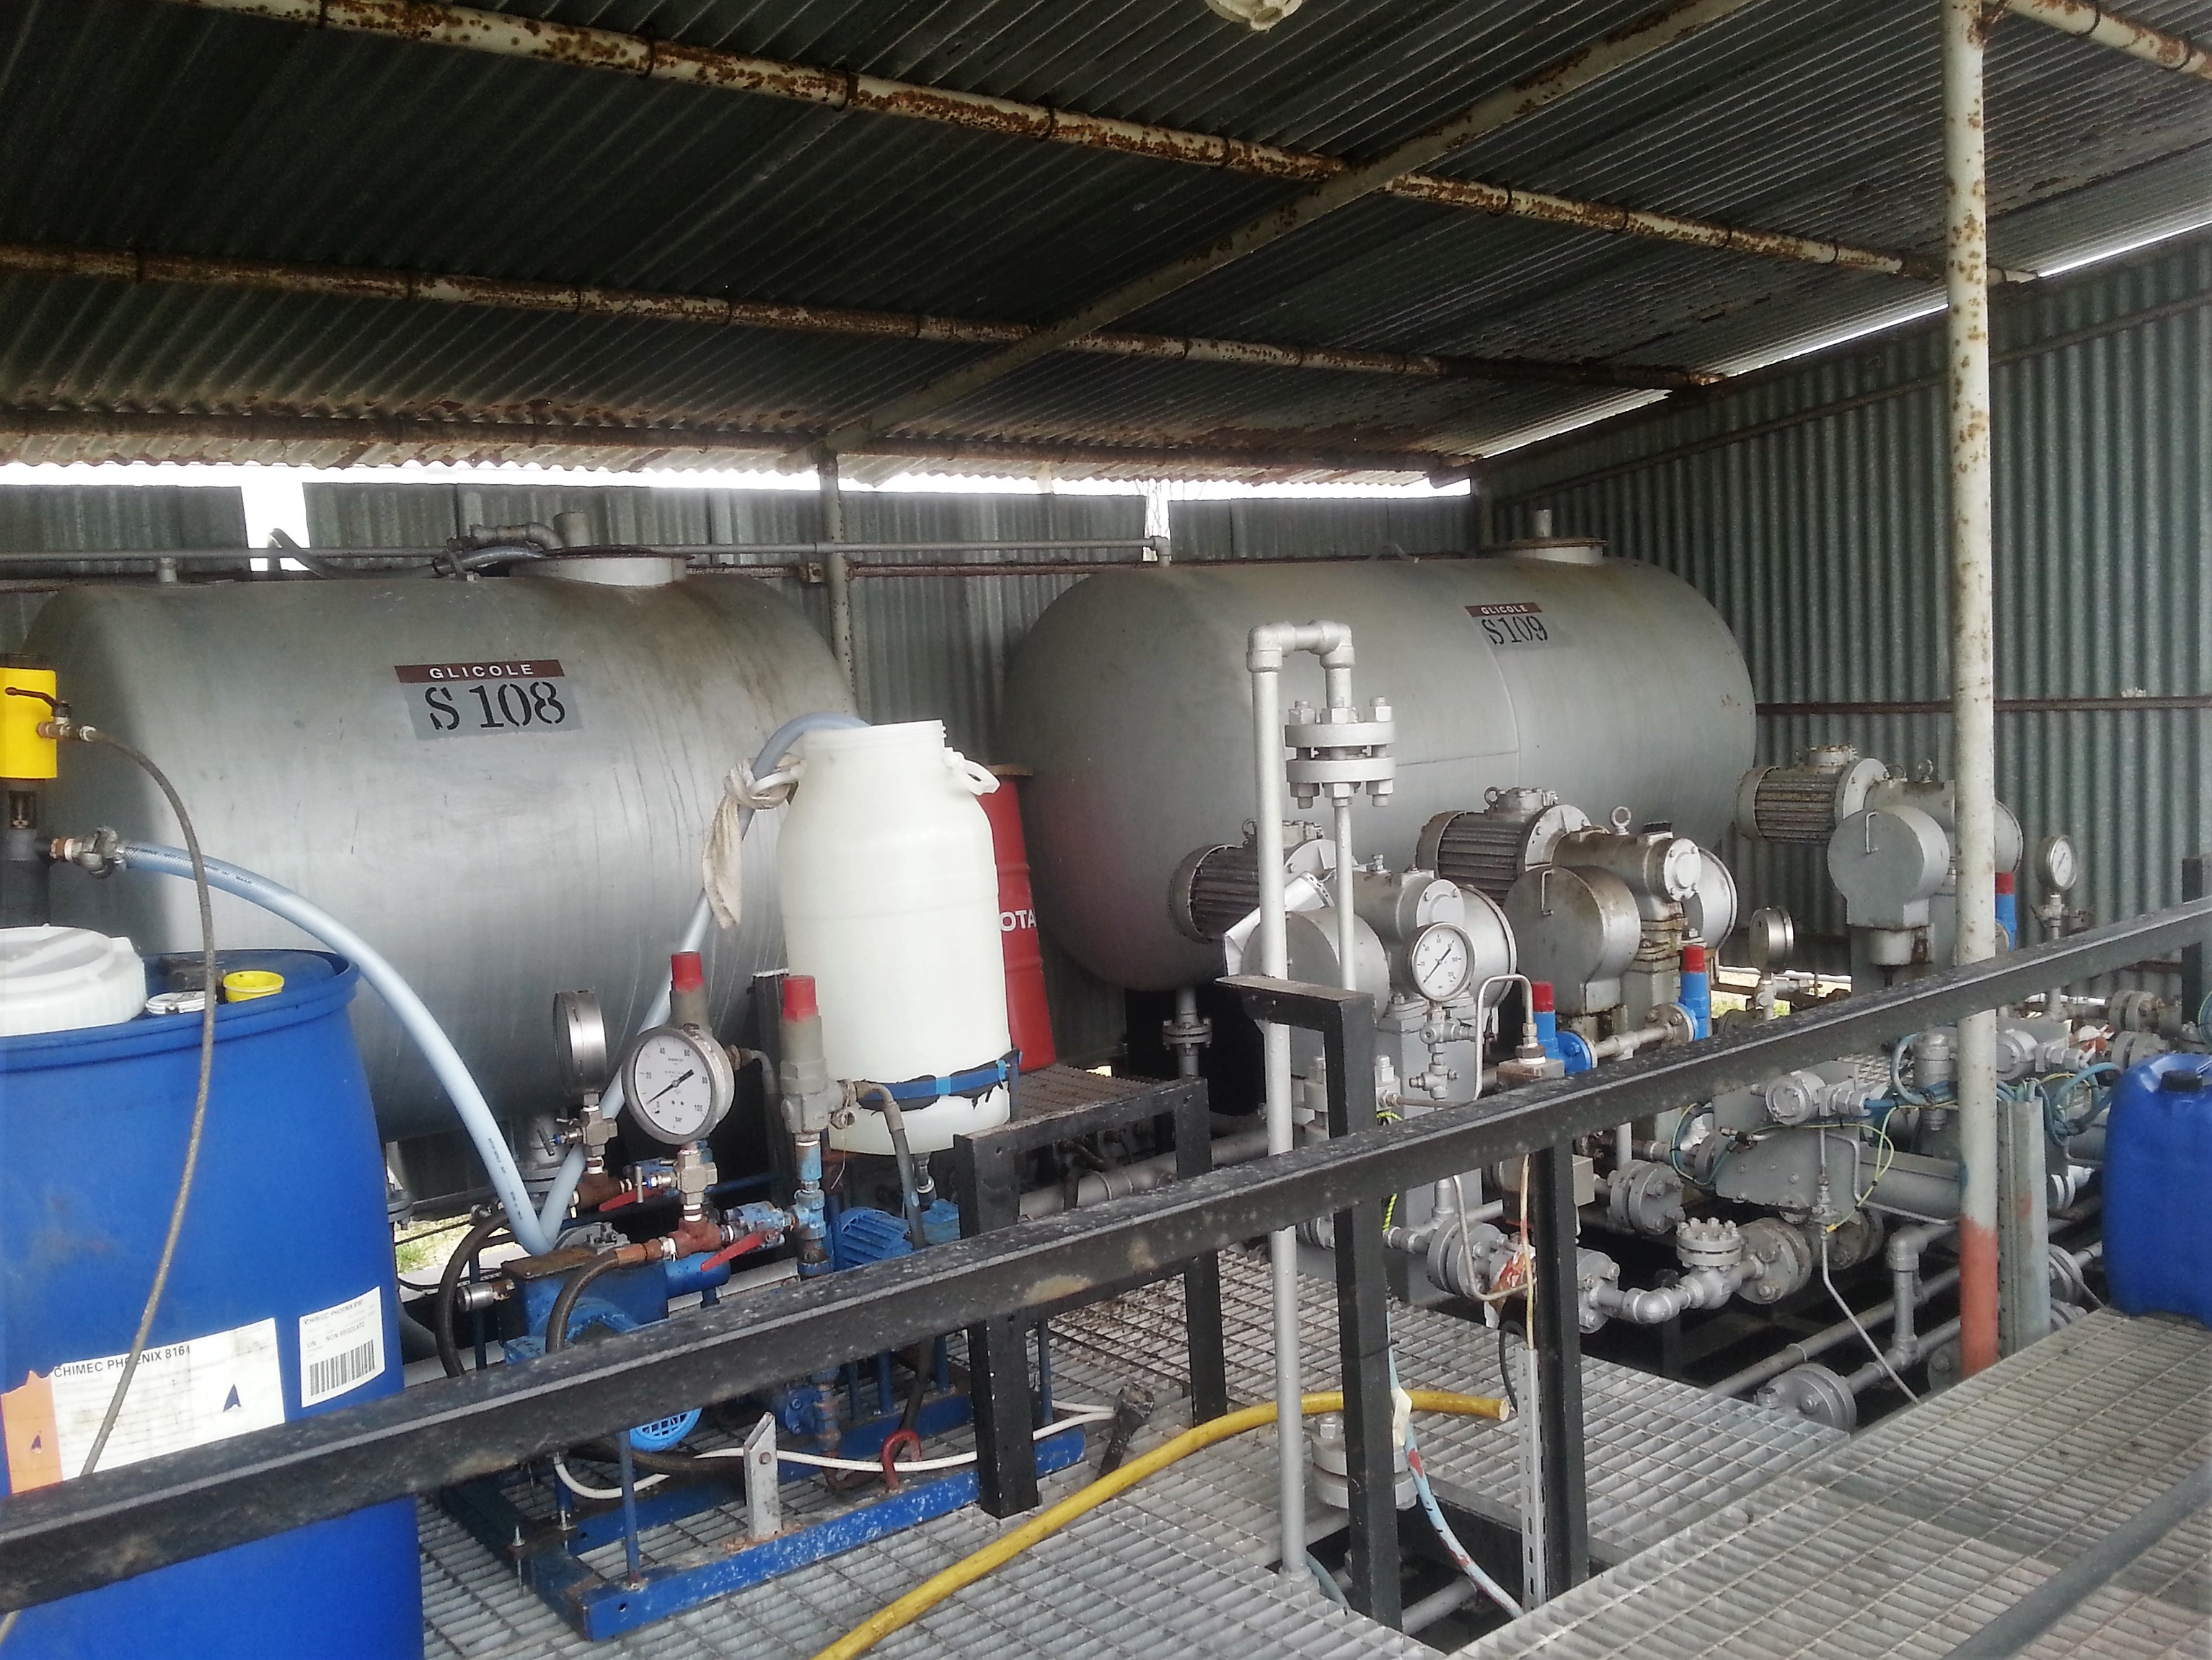
\includegraphics[width=\textwidth]{fig/test/centrale/glicol1.jpg}
    \caption{Pompe dosatrici per iniziezione di glicol.} 
    \label{fig:glicolpump}
\end{figure}
\paragraph{Riscaldatori}
\paragraph{Filtri}

\subsubsection{Sicurezza}
\paragraph{Sicurezza degli impianti di processo}
\paragraph{Sicurezza detenzione gas}
\paragraph{Rilevazione incendio}
\paragraph{Sistema antincendio}

\subsubsection{Utenze}
\paragraph{Rete elettrica}
L'energia elettrica arriva in centrale alla tensione di 10 kV e viene convogliata al quadro a media tensione (QMT-1), previsto per una tensione nominale di 10/20 kV, 50 Hz in sistema trifase a neutro isolato. Il quadro è costituito da un arrivo e due partenze, da cui sono alimentati due trasformatori da 800 kVA, i quali convertono la tensione a 380 V. La corrente passa infine dai trasformatori al quadro a bassa tensione tramite cavo unipolare. Per l'alimentazione degli ausiliari è previsto un raddrizzatore con relativa batteria di accumulatori. L'impianto luce è collegato con un trasformatore a monte da 30 kVA che converte la tensione da 380 V a 220 V. In caso di
\paragraph{Sala controllo}

\subsection{La linea Verdicchio}

\section{Configurazione sperimentale: materiali e modalità di esecuzione}
\sectionmark{Configurazione sperimentale}
\subsection{Schiumogeno}
Il prodotto CHIMEX Phoenix 6163 è uno schiumogeno; disciolto in acqua, fa diminuire notevolmente la tensione interfacciale che compete alla superficie di separazione fra la soluzione diluita così ottenuta e la fase gassosa.
\subsection{Antischiuma}
Il prodotto CHIMEC Phoenix 8161 è un antischiuma che favorisce l'avanzamento della schiuma a valle del separatore, con conseguenze decisamente negative sull'impianto.

\subsection{Punto di iniezione - San Marco}

\begin{figure}[!htbp] %Immagine layout di mandata
    \centering
    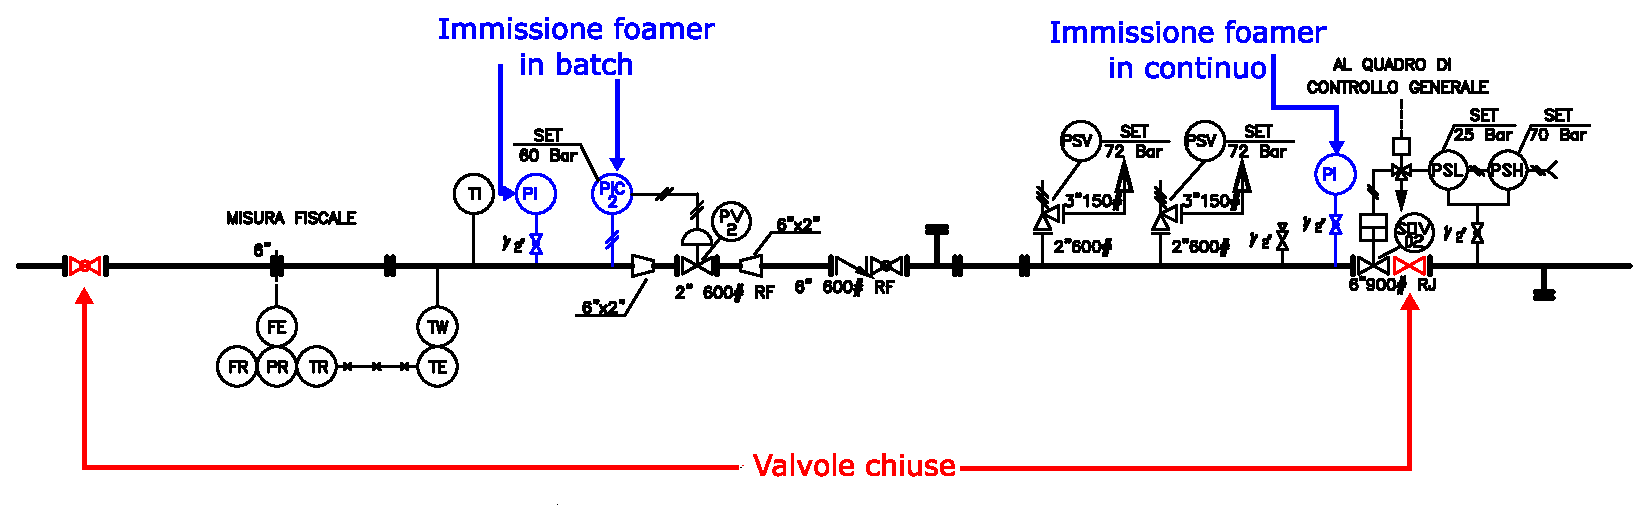
\includegraphics[width=\textwidth]{fig/test/mandata.eps}
    \caption{Layout linea di mandata SNM, modalità di applicazione del batch.} 
    \label{fig:mandata}
\end{figure}

\subsection{Apparati di misura}
\subsection{Iniezione in-batch}
\subsection{Iniezione in continuo}

I parametri di pressione e temperatura sono stati monitorati tramite un termomanometro digitale installato sulla linea di mandata, tra la Fisher e le valvole di blow-down, in corrispondenza dei due spool flangiati. Il defoamer è stato iniettato all'ingresso del separatore con una portata di 30 litri orari, in continuo, tramite l'utilizzo di pompe dosatrici già presenti alla centrale SGM ((\figurename~\ref{fig:glicolpump}).

\section{Risultati e discussione}
\subsection{Studio degli effetti a breve termine}
\subsection{Andamento produttivo post-test}
\subsection{Analisi costi e benefici}
\subsection{Pigaggio della linea di produzione}